\documentclass[12pt, titlepage=true, toc=bib]{scrartcl}


%Deutsche Silbentrennung
%Trennung von Wörtern mit Umlauten
%Deutsche Sprachregeln
\usepackage[utf8]{inputenc}
\usepackage[T1]{fontenc}
\usepackage[english]{babel}

%Schriftart
\usepackage[bitstream-charter]{mathdesign}
\usepackage[activate={true, nocompatibility}, final, tracking=true, kerning=true, spacing=true, factor=1100, stretch=10, shrink=10]{microtype}
%Selbe Schriftart für Überschriften												
\addtokomafont{disposition}{\normalfont\bfseries}

\usepackage{amsmath}

%Zeilenabstand							
\usepackage[onehalfspacing]{setspace}

%Literaturverwaltung
\usepackage[backend=biber, style=authoryear, date=year, doi=false, isbn=false, url=false, maxcitenames=2, maxbibnames=8]{biblatex}		
%Formatierung für Anführungszeichen
\usepackage[autostyle]{csquotes}
%u.a. in et al. umwandeln
\DefineBibliographyStrings{ngerman}{andothers = {{et\,al\adddot}},}
%Formatiert die Zitationsklammern
\renewcommand{\labelnamepunct}{\addcolon\addspace}
\renewcommand{\postnotedelim}{\addcolon\addspace}
\DeclareFieldFormat{postnote}{#1}
\DeclareFieldFormat{multipostnote}{#1}
%Leerzeile zwischen den Einträgen im Literaturverzeichnis
\setlength{\bibitemsep}{0.5\baselineskip plus 0.5\baselineskip}
%Schrägstrich bei zwei Autor*innen
\renewcommand{\multinamedelim}[0]{/}
\renewcommand{\finalnamedelim}[0]{/}
%URL bei Artikel- und Büchereinträgen entfernen
\DeclareSourcemap{
  \maps[datatype=bibtex]{
    \map{
      \pertype{article}
      \pertype{book}
       \step[fieldset=url, null]
    }
  }
}


\addbibresource{HA_SNA.bib}

%Seitenränder
%\usepackage[right=4	cm,]{geometry}

%Paket, um Grafiken einzubinden
\usepackage{graphicx}
%\usepackage{float}
%Paket, um Grafiken davon abzuhalten, außerhalb bestimmter grenzen zu floaten [section]: verbietet gleiten außerhalb der Section
%\usepackage[section]{placeins}
%zum Formatieren der Bildunterschriften
\usepackage{caption}
\captionsetup{format=plain, indention=0cm, justification=justified, singlelinecheck=off, width=.95\linewidth, font={small, singlespacing}}
%\captionsetup[table]{name=Tab. }
\setkomafont{captionlabel}{\bfseries}

%Wird für das r-Paket stargazer benötigt
\usepackage{dcolumn}

%Listen
%\usepackage{enumitem}

%pdf-Dateien einbinden
%\usepackage{pdfpages}

%Anhang ohne Seitenzahl im ToC
%\makeatletter
%\let\partbackup\l@part
%\renewcommand*\l@part[2]{\partbackup{#1}{}}
%\makeatother

%\clubpenalty = 10000
%\widowpenalty = 10000
%\displaywidowpenalty = 10000

%Verlinktes ToC
\usepackage[colorlinks, pdfpagelabels, pdfstartview=FitH, bookmarksopen=true, bookmarksnumbered=true, linkcolor=black, urlcolor=black, plainpages=false, hypertexnames=false, citecolor=black]{hyperref}



\begin{document}

\titlehead{\flushleft{University of Copenhagen\\
			Department of Political Science\\
			Social Network Analysis (ASTK18106U)\\
			Yevgeniy Golovchenko
			}}
\author{Ole Fechner, Johannes Kopf}
\title{Structure and Strategy of the Internet Research Agency on Twitter}


\date{\normalsize{Copenhagen, \today}}

\publishers{\flushleft{\normalsize{Boddinstr. 15\hfill Moselstr. 50\\
							 12053 Berlin\hfill 50674 Cologne\\
							 ole.fechner@fu-berlin.de\hfill jkopf@posteo.de\\
							 MA Political Science\hfill MA Political Science}}}

\maketitle[0]

\newpage

\thispagestyle{empty}
\tableofcontents

\newpage

\thispagestyle{empty}
\listoftables

\newpage

\thispagestyle{empty}
\listoffigures

\newpage
\setcounter{page}{1}

\section{Introduction}

``Frankly, the United States is under attack'', said Dan Coats, director of U.S. National Intelligence in an interview concerning the influence of Russian troll accounts on the social network Twitter in the 2016 U.S. presidential elections (\cite{popken_twitter_2018}). What seems to be a drastic statement is supported by Twitter committing a list of 2,857 supposedly Russian troll accounts connected to the state-sponsored Internet Research Agency (IRA) to the U.S. Congress. Coats expects Russia ``to continue using propaganda, sympathetic spokesmen, and other means of influence to [...] exacerbate social and political fissures in the United States'' (\cite{popken_twitter_2018}). With its low cost and risk, as its free to use and difficult to trace back, Twitter appears especially attractive as a means to gain influence in foreign countries. The IRA exhibits a high degree of professionalism, that should not be underestimated: their workers are divided in day and night shifts, to be able to post in different US time zones; are trained in English grammar and US holidays; had quotas to meet; and have their activity monitored (\cite{kirby_what_2018}). This indicates an intentional strategy, an orchestrated act of state-institutional interference in a foreign election, that urges for an analysis. Given the importance of the matter, research on the activity of Twitter trolls promises shedding some light on an issue of growing importance for everyday politics.
\marginpar{JK}

Given the recency of the IRA's exposure through journalists, only few researchers have approached the topic and already published their results. See (\cite*[]{golovchenko_state_2018}) for an analysis of the information warfare on Twitter regarding Ukraine, or \textcite{stewart_examining_2018} for an analysis of trolls and polarization in a retweet network). Linvill and Warren (\cite*{linvill_troll_2018}) present an early analysis of the IRA using a sequential mixed method design, first qualitatively categorizing the Twitter accounts into groups and subsequently examining those account's activity over time. This paper seeks to build upon Linvill and Warren's work by further investigating potential differences in troll behavior between various communities of trolls. Our research question is as follows: how does IRA troll account behavior differ between the Twitter communities they engage in? As a theoretical foundation, we rely on the concepts of agenda-building and astroturfing, assuming strategic activity and behavior of Russian trolls in trying to gain influence on Twitter. We are using a dataset consisting of 147,428 retweets by 453 trolls, which includes a large share of trolls who have been already qualitatively categorized by Linvill and Warren. We apply a Social Network Analysis (SNA), building an ego-centered retweet network using retweets as ties between different Twitter accounts as nodes. After establishing the nature of the network the network, we calculate different network properties to understand its structure. First, we are running a community detection algorithm to cross-validate Linvill and Warren's findings. Second, we analyze the graph densities in those different communities, to understand how the IRA engages within them. Third, we compute out- and indegrees for the nodes, to further investigate support for different account behavior across communities. Finally, we compute different k-cores, to analyze the overall most active and inter-connected community of trolls. We then discuss the findings with a focus on the mechanics of information spreading and the limitations of our SNA approach with regard to the network being ego-centered.


\section{Agenda-building and astroturfing}

The process of trying to move an actor's agenda to the agenda of other actors, especially policymakers, is defined as \textit{agenda-building} (\cite[3]{linvill_troll_2018}). This can be extended to the question of how the public views certain issues, usually by analyzing media coverage of those issues: ``Agenda-building research examines how certain groups, such as those in politics and business, influence what issues journalists cover as well as how the public views issues'' (\cite[434]{parmelee_agenda-building_2014}). Since the rise of social media platforms like Twitter and Facebook, agenda-building has been taking place in those environments. This is due to journalists drawing heavily on Twitter for their job and, as well as, Twitter being the most popular social media platform for participating in political discussions, which from there are often taken to other media (\cite[435, 437]{parmelee_agenda-building_2014}). Influencing the citizens of another country through the use of media is nothing new, rather it is used in conflicts or during war regularly. ``However, Russia's work on social media has taken agenda-building efforts by nations into a new context'' (\cite[3]{linvill_troll_2018}).
\marginpar{OF}

Closely linked to agenda-building is a second phenomenon called (political or/and online) \textit{astroturfing}, which can be characterized as the ``creation of a false or exaggerated impression of grassroots support'' (\cite{harcup_astroturfing_2014}). It describes the strategic and coordinated approach of a group with the aim to create the impression of a certain public opinion, that otherwise might not exist in this form. On social media, those groups use many different accounts, posting and interacting with regular users to create the desired impression. For the purpose of this paper, astroturfing will be seen as a strategy of agenda-building, since its use by the IRA showed to be successfully able to influence the public discourse in their desired manner. The anonymity provided by platforms like Twitter, as well as the covert structure of those groups, make them very hard to discover (\cite[564]{yang_how_2017}). Instead of the presumed agenda behind the organization, this exploratory study will take the structure of the IRA as a starting point. Social Network Analysis, which will be introduced in the next section, offers an excellent tool box to conduct this task.


\section{The social network analysis (SNA)}

To analyze the structure and possible strategies of the IRA, we employ a Social Network Analysis (SNA), due to it being strongly data-driven and having few theoretical assumptions -- the notion of people relating to each other, and the significance put into the structure and strength of those relations being almost the only ones (\cite[982]{golovchenko_state_2018}) -- makes it especially viable for our exploratory approach. SNA conceptualizes the linkages between actors as \enquote{channels for transfer or \enquote{flow} of resources}, while the actors themselves are seen as ``interdependent rather than independent, autonomous units'' (\cite[4]{wasserman_social_1994}). Therefore, the different actor attributes are theorized as emerging out of their relations and not vice versa, as in most other types of quantitative analyses (\cite[8]{wasserman_social_1994}). This allows us to oversee the problematic regarding the intentions of actual people behind varying accounts and enables us to focus on the structure and strategy of the IRA. The most important relation to analyze how the IRA uses astroturfing as a strategy for agenda-building is the distribution of information, in this case via retweets. Accordingly, the basis of this paper will be a social network consisting of Twitter accounts as nodes and retweets as edges (or linkages).
\marginpar{OF}


\subsection{Data: An ego-centered retweet network}

We will use a dataset, published by NBC News (\cite*{popken_twitter_2018}), consisting of 203,451 Tweets by 453 accounts between July 2014 and September 2017, which were linked to the IRA by an official document handed over to US Congress by Twitter. Twitter justifies this linking by referring to ``third party sources'', which makes it impossible to reconstruct or evaluate their method. We therefore have to assume those accounts' links to the IRA to be correct, as it is the best evaluation available.
\marginpar{JK}

To create the social network, we need to clean the data: First, we drop any of the tweets that are not retweets, which leaves us with 147,428 retweets by 453 troll accounts; 120 trolls, who did not retweet and were not retweeted by others, were dropped accordingly. Our dataset now consists of a set of 333 unique troll Twitter handles\footnote{A Twitter handle is the screen name of a Twitter account that can be changed by the users.}; a variable stating the unique User ID is used to validate the absence of duplicates. Since we only have information of these 333 accounts retweeting other users, but not of other users retweeting them, the network is ego-centered around the group of trolls.\footnote{Wassermann and Faust define ego-centered networks as follows: ``An ego-centered network consists of a focal actor, termed ego, as set of alters who have ties to ego, and measurements on the ties among these alters'' (\cite[42]{wasserman_social_1994}). The network in this paper is based around a set of egos (the sending trolls), while the other users can only have ties to the set of egos.} Of these 333 trolls, 151 (ca 45\%) are both sender and receiver, while the other 182 (ca 55\%) are only sender.\footnote{We define a retweet sender as the person retweeting an original Tweet by another person, who, accordingly, is the retweet receiver.} A third group of 71 trolls, who are only receivers, was found by inspecting who was retweeted by the original group of trolls, thus increasing the total number of trolls to 404. Finally, the biggest chunk of nodes in the dataset consists of 36,485 users, who are retweeted by the trolls, but are not themselves categorized as trolls by Twitter. Table~\ref{tab:userstat} gives a first overview of the dataset. Overall, there are 36,889 unique twitter users in the dataset, 404 classified trolls and 36,485 non-trolls. The retweets contain relational information about one user retweeting another, therefore creating a directional edge between the two. Thus, the graph is a directed, ego-centered network of 333 IRA accounts with 36,889 unique Twitter accounts as nodes and edges representing retweets from the sender to the receiver.

\begin{table}[!ht] \centering 
\begin{tabular*}{.95\linewidth}{@{\extracolsep{\fill}} lrrr} 
\\[-1.8ex]\hline 
\hline \\[-1.8ex] 
User & N & Senders & Receivers \\ 
\hline \\[-1.8ex] 
Troll & 404 & 333 & 222 \\ 
Non-Troll & 36,485 & 0 & 36,485 \\ 
Total & 36,889 & 333 & 36,707 \\ 
\hline \\[-1.8ex] 
\end{tabular*} 
  \caption[User Statistics]{Distribution of troll accounts and retweet senders and receivers in the data.}
  \label{tab:userstat} 
\end{table} 

To further extend our data and our scope of analysis, we are adding qualitative information on the IRA trolls, provided through a dataset by Darren Linvill and Patrick Lee Warren (\cite*{linvill_troll_2018}) via the online news outlet FiveThirtyEight (\cite{roeder_why_2018}). Linvill and Warren conducted a qualitative analysis, categorizing a sample of 1,133 IRA troll accounts by examining the tweet content and the account names, applying a temporal analysis of the trolls tweeting behavior after. They ``identified five categories of IRA-associated Twitter handles, each with unique patterns of behaviors: \textit{Right Troll}, \textit{Left Troll}, \textit{Newsfeed}, \textit{Hashtag Gamer}, and \textit{Fearmonger}'' (\cite[6]{linvill_troll_2018}). In addition, there are three categories, which are not used within their analysis: \textit{Non-English}, \textit{Commercial} and \textit{Unknown}. The categories \textit{Right Troll} and \textit{Left Troll} need little explanation, as they include users who are described as broadcasting right-leaning populist and socially liberal messages. \textit{Hashtag Gamers} are users who are playing word games on Twitter, mostly non-political, though sometimes including left- or right-leaning messages. \textit{Newsfeed} Trolls are posing as local US News Agencies, mostly linking to legitimate news content, often with a pro-Russian perspective. Fearmongers spread news of crisis events such as Tweets about salmonella infections. The \textit{Non-English} troll category includes users who tweeted in other languages than English, predominately Russian, some German and little French and Spanish. \textit{Commercial} Trolls are not included in our dataset. Finally, users were categorized as \textit{Unknown}, if they could not be assigned to other categories for lack of information in their tweets. These categories will be included in this paper's analysis, since might be interesting to see how they interact with the other trolls. We are appending Linvill and Warren's account categories to our data, finding categories are available for 394 of the 404 troll handles in our dataset, meaning that around 98\% of the trolls in our dataset are categorized. Table~\ref{tab:trollstat} shows the distribution of the categories among our dataset.

\begin{table}[!ht] \centering 
\begin{tabular*}{.95\linewidth}{@{\extracolsep{\fill}} lrrrr} 
\\[-1.8ex]\hline 
\hline \\[-1.8ex] 
Category & N & Senders & Receivers & Average followers \\ 
\hline \\[-1.8ex] 
Right & 101 & 75 & 90 & 4649 \\ 
Left & 110 & 104 & 48 & 1783 \\ 
Hashtag Gamer & 61 & 43 & 60 & 3021 \\ 
Non-English & 106 & 100 & 7 & 2127 \\ 
Newsfeed & 11 & 1 & 10 & 16446 \\ 
Fearmonger & 4 & 0 & 4 & 0 \\ 
Unknown & 11 & 10 & 3 & 3306 \\ 
Total & 404 & 333 & 222 & 4476 \\ 
\hline \\[-1.8ex] 
\end{tabular*} 
  \caption[Troll Statistics]{Distribution of account types categorized by Linvill and Warren (2018)}
  \label{tab:trollstat} 
\end{table} 
 
As another attribute, we are appending information on the count of followers of the troll accounts from a second dataset provided by NBC news. The information on the count of followers provided only includes one figure and does not vary over time, without specification of when these follower counts were obtained. We will thus only use them as a heuristic to compare different accounts within groups. Table~\ref{tab:trollstat} gives the average number of followers for each account category. Finally, we are using the full time period of retweets, from July 2014 to September 2017. This paper is not interested in a time period preceding a specific event, like an election or a specific trending discussion, but rather strategic behavior of the trolls in general. Therefore, we include all of the tweets in the data into the network, thus disregarding their date.


\subsection{Methods}

To understand the IRA's division of labor, we begin with testing if Linvill and Warren's qualitative findings of the different account types would be reproducible via network properties. To achieve this, we will draw on a community detection algorithm based on modularity, known as the Louvain Method (\cite{blondel_fast_2008}).\footnote{For our network, this algorithm produced the best results. The Infomap algorithm (\cite[cf.][]{rosvall_maps_2008}) results in one big community containing ca 98\% of the nodes.} Communities are mesoscopic structures of a graph, that consist ``of a group of nodes that are relatively densely connected to each other but sparsely connected to other dense groups in the network'' (\cite[1083]{porter_communities_2009}). The Louvain algorithm is based on modularity, ``which attempts to measure how well a given partition of a network compartmentalizes its communities'' (\cites[1088]{porter_communities_2009}[cf. also]{blondel_fast_2008}). It approximately optimizes the modularity for each partition, thus identifying communities. We will compare the communities with Linvill and Warren's account types to see if we can better understand the identified community structure.
\marginpar{OF}

One important measure for the cooperation of the accounts is graph density, the proportion of all possible edges that are present in the graph (\cite[101]{wasserman_social_1994}). Since the network is ego-centered, it only makes sense to calculate density for the troll subgraph. Following Wassermann and Faust (\cite*[102]{wasserman_social_1994}) we calculate the density of the different community subgraphs \( \Delta_{c} \) as: \[ \Delta_{c} = \frac{2L_{c}}{g_{c}(g_{c} - 1)} ,\] where \( L_{c} \) is the number of edges present in the community subgraph, and \( g_{s} \) is the number of nodes in said graph. We will compute density for the directed graph, as well as for its undirected version.\footnote{To create the undirected graph, we keep an edge for every one-directional tie, and collapse all reciprocal ties into one tie, thus avoiding multiple ties in one relationship.} We will then compare the densities of the different communities, which can give an indication weather the IRA has distinctive strategies for those groups. In communities with higher density, the accounts are cooperating more closely, meaning they spread information further through retweeting, while accounts in less dense communities rely more on information they put into the network themselves.

Identifying the most important accounts helps to understand the structure of the IRA. Operationalizing importance in SNA is usually achieved through centrality and prestige indices, whereas not only the chosen actors are considered prestigious, but also those doing the choosing (\cite[170]{wasserman_social_1994}). To show the most central accounts, we will calculate outdegree. The index can only be computed for IRA accounts, since -- because of it being ego-centered -- they are the only ones retweeting in our dataset. We will calculate the outdegree weighted and unweighted respectively.\footnote{A weighted graph is a graph in which each edge carries a value (\cite[140]{wasserman_social_1994}), in this case the number of retweets between two accounts. In an unweighted graph, each edge has the value 1.} The weighted outdegree results in the number of different unique accounts the user retweeted, the unweighted outdegree gives the number of total retweets of the user as a result. The outdegree of a node \( d_{out}(n_{i}) \) is computed as \[ d_{out}(n_{i}) = \sum_{j} x_{ij} ,\] where \( x_{ij} \)\footnote{Note that in- and outdegree are calculated for directed graphs, hence \( x_{ij} \neq x_{ji} \).} is an edge from \( i \) to \( j \) (\cite[cf.][178]{wasserman_social_1994}). For the weighted outdegree \( x_{ij} \) is multiplied by the value of the edge. Prestige, on the other hand, will be calculated through indegree, which results in those accounts retweeted the most and can therefore tell about what accounts the IRA draws on. It will also be computed for the weighted and unweighted graph separately, which shows the number of different accounts that retweeted the user, and how often the user got retweeted in total respectively. The indegree of a node \( d_{in}(n_{i}) \) is computed simply as \[ d_{in}(n_{i}) = \sum_{j} x_{ji} ,\] where \( x_{ji} \) is an edge from \( j \) to \( i \) (\cite[cf.][202]{wasserman_social_1994}). For the weighted outdegree \( x_{ji} \) is multiplied by the value of the edge. Although we can calculate the prestige for all accounts, the numbers can only tell us which accounts are prestigious for the trolls.

Finally, we will look at the most engaged users in the network to identify the so-called super-spreaders of information. In SNA, the ability to spread information better than other individuals is ascribed to their unique location in the network, which makes identifying those a prime task of analyzing networks used for false information (\cite[1]{pei_searching_2015}). Pei et al. (\cite*{pei_searching_2015}) show that, compared to other approaches, the k-core method predicts the super-spreaders most accurately. \enquote{A k-core is a maximal subset of the network where all nodes are connected to at least \enquote{k} number of other nodes} (\cite[983]{golovchenko_state_2018}). We can define a subgraph \( G_{s} \) as a k-core if \[ d_{s}(i) \geq k \text{ for all } n_{i} \in N_{s} ,\] where \( d_{s}(i) \) is the (in-)degree of node \( i \) and \( N_{s} \) the set of nodes in the subgraph (\cite[266]{wasserman_social_1994}). Hence, the k-core specifies a subgraph via the number of ties that must be present between nodes, it is based on the nodal degree. The network being ego-centered limits the validity of the results, since every non-troll in reality has a higher degree through retweets from other non-troll accounts and retweeting themselves. We can therefore only identify the most important IRA accounts regarding their own network. To account for this, we will also compute the k-in-core through the indegrees. The idea is that information from one account is spread quickly, if this account is retweeted a lot and the accounts retweeting it also get retweeted a lot.


\section{Analyzing the IRA retweet network}

In the preceding chapter, the data and methods forming the base of our analysis have been introduced. Figure~\ref{fig:graph} shows the entire retweet network consisting of three main clusters. We will focus our analysis on those clusters in four steps. First, the results of the modularity community detection algorithm are illustrated and new communities are established, based on our findings, as well as the qualitative coding of Linvill and Warren. Secondly, graph densities are compared between these communities. Thirdly, degree centrality indices are analyzed for the whole graph to identify the most active IRA accounts and the most prestigious accounts. Finally, we will take a look at the k-cores, to detect information super-spreaders and the connection between the clusters. In the last section, we discuss the findings regarding the strategy and structure of the IRA.
\marginpar{JK}

\begin{figure}[!ht]
\centering
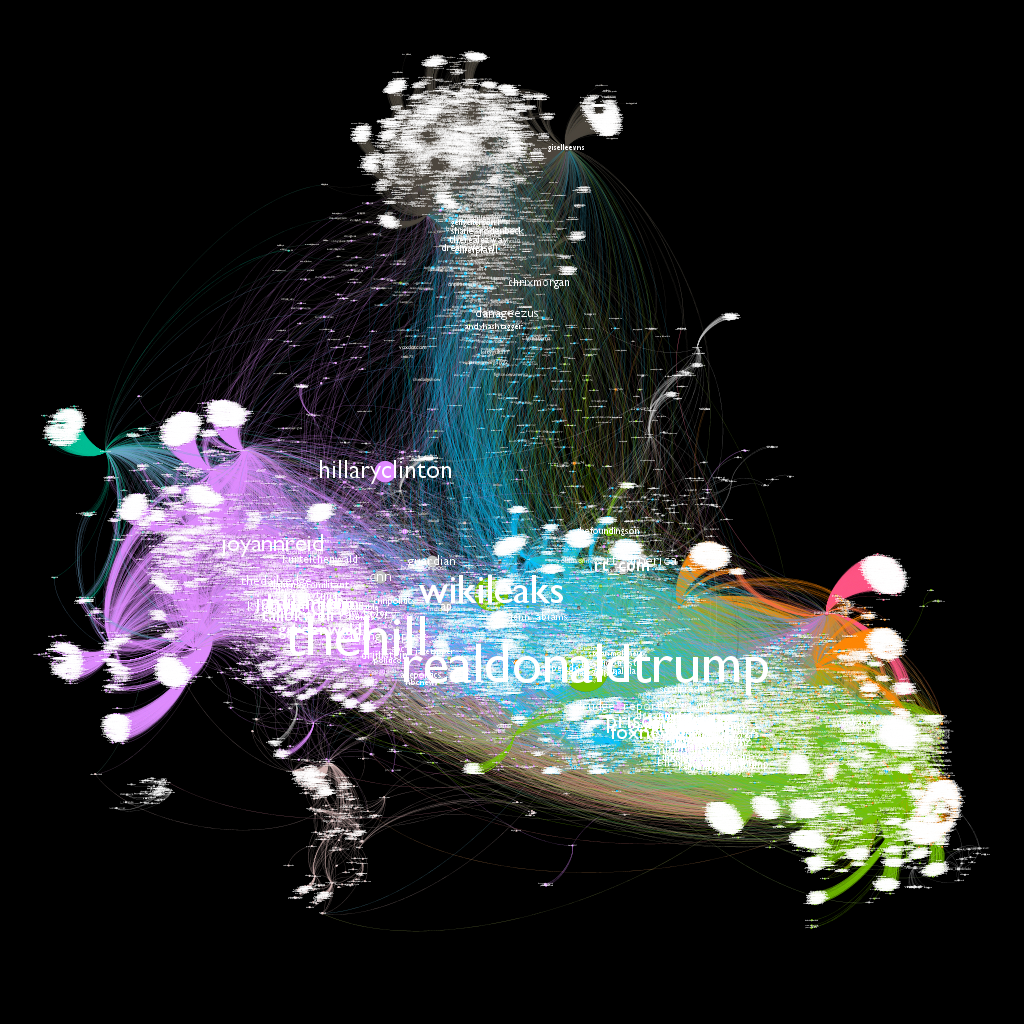
\includegraphics[width=0.95\linewidth]{Network_modularity.png}
\caption[Retweet network]{The entire retweet network. Nodes represent profiles, while a connection represents at least one retweet between them. Node and label size represent popularity (indegree). Colors represent the communities detected by the Louvain algorithm.}
\label{fig:graph}
\end{figure}


\subsection{Findings}

We run a modularity-based community detection, following the Louvain Method. Figure~\ref{fig:distcom} shows the distribution of algorithm communities among the qualitative account categories created by Linvill and Warren (\cite*{linvill_troll_2018}). For further analysis, we rely on communities that were computed with the Louvain Method, since they originate from the structure of ties within our dataset and this appears to be more consistent with the methodology of SNA. Not to exceed the scope of this paper, we focus only on the three largest communities, while combining the rest to a single category: \textit{other}. We then apply the qualitative categorization to the new found communities. In Figure~\ref{fig:distcom}, we see that some categories overlap strongly with distinct communities, whereas other categories show a rather mixed composition in our data. 94\% of the left troll category is captured with one community,  making up our new left troll community. The hashtagger community is 90\% captured by one community, making up our new hashtagger troll community. 90\% of the right troll category is made up by two major communities with shares of 52\% and 38\%, which we merge to one new right troll community. Such a merger is justified by the argumentation, that the mentioned two communities could represent distinct right-wing groups underneath a general right-wing community (e.g. Conspiracy Theorist vs. Alt Right User) (\cite[cf.]{kaiser_unite_2018}). These categories, overlapping with at least 90\%, offer sufficient congruence to continue using the qualitative attributes. The non-english troll category consists of multiple communities, with a biggest community share making up 27\%. All of the non-english and other categories consist mainly of smaller communities, which leaves us with four distinct communities: \textit{Right Troll}, \textit{Left Troll}, \textit{hashtagger} and \textit{Other}. It is important to note, that the algorithm puts some nodes in a different category than Linvill and Warren, which bears the risk of having biased results. However, the occurrence of partial bias appears inevitable due to the detected incongruence of the account categorization within the detected communities. In Figure~\ref{fig:distcat} the distribution of account categories among our new communities is depicted, which illustrates the potential bias.
\marginpar{JK}

\begin{figure}[!ht]
\centering
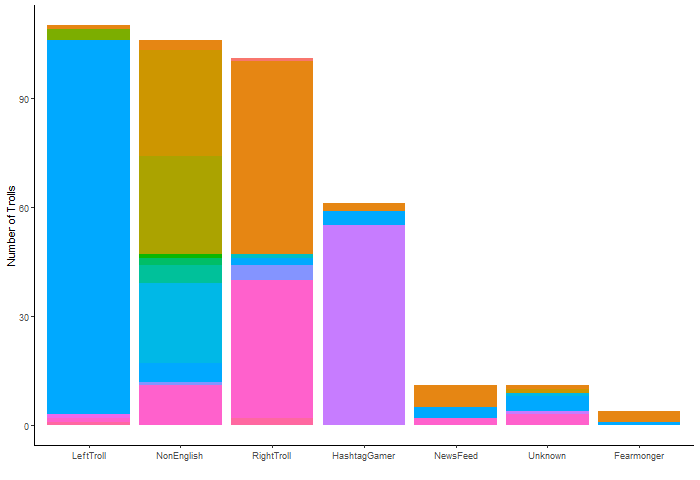
\includegraphics[width=0.95\linewidth]{final_figure1.png}% die Breite des eingefügten Bildes entspricht 95% einer Zeilenlänge
\caption[Distribution of communities among account categories]{Color reflects communities detected by the Louvain Method among account categories by Linvill and Warren.}
\label{fig:distcom}
\end{figure}

\begin{figure}[!ht]
\centering
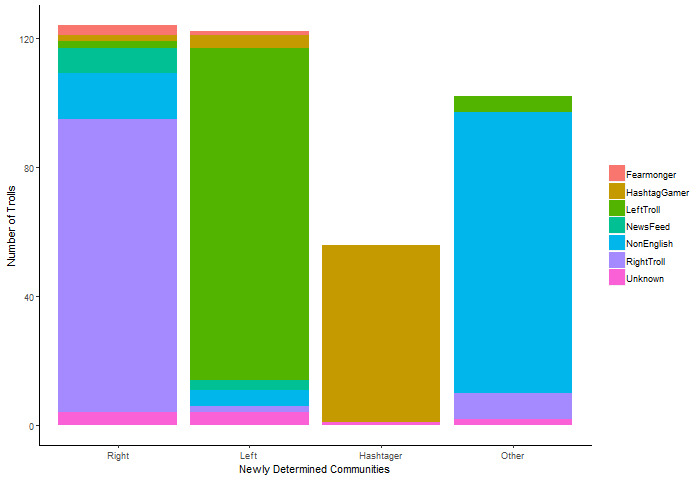
\includegraphics[width=0.95\linewidth]{final_figure2.png}% die Breite des eingefügten Bildes entspricht 95% einer Zeilenlänge
\caption[Distribution of account categories among communities]{Distribution of account categories among communities detected by the Louvain Method. Color reflects account categories by Linvill and Warren.}
\label{fig:distcat}
\end{figure}

Next, the graph densities are calculated: Figure~\ref{fig:dens} shows the graph densities for the three communities, both directed and undirected versions of each subgraph. We see that the undirected subgraphs' densities are approximately twice as high as directed ones, with only minor deficits. Bearing in mind the mode of creating the undirected graph, this can be interpreted as a lack in reciprocal ties among the subgraphs. If there was a considerable amount of reciprocal ties, this would cause a higher density of the directed subgraph in comparison to the undirected one (>50\%).

\begin{figure}[!ht]
\centering
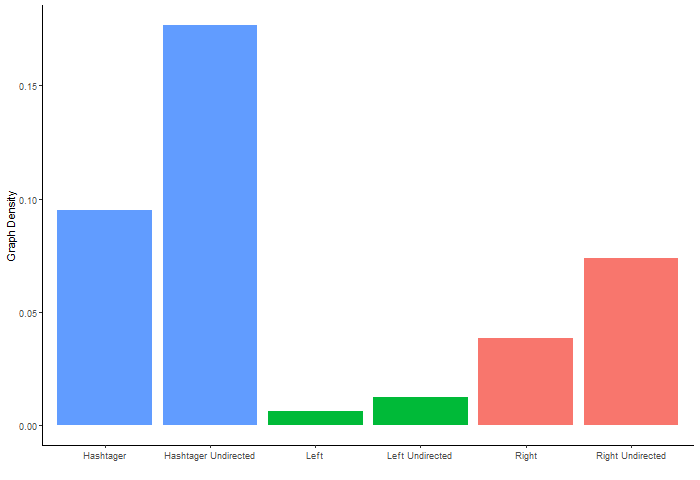
\includegraphics[width=0.95\linewidth]{final_figure3.png}
\caption[Graph densities]{Graph densities in the three biggest communities.}
\label{fig:dens}
\end{figure}

Examining the magnitude of densities across different community subgraphs, we find that the hashtagger community is by far the most dense. Approximately 17.7\% of all possible ties are present for the undirected subgraph, relating to this community's nature of retweeting one another and playing word games. Hence, it appears to constitute this community's cohesion to retweet one another frequently. Right trolls have the second largest density with 7.4\%. In respect to the numbers for the undirected graphs, this shows the right trolls to have more than six times the density of the left, who merely show to have one of 1.2\%.

We now analyze the degree centrality of our graph starting with the outdegree, which we use as a measure for centrality and the weighted outdegree, which gives additional information on the activity of the user. Because of our network is ego-centered around the central group of trolls, only troll accounts have outdegrees. Table~\ref{tab:out} shows the top 10 users ranked by outdegree.

\begin{table}[!ht] \centering 
\begin{tabular*}{.95\linewidth}{@{\extracolsep{\fill}} lrrrrr} 
\\[-1.8ex]\hline 
\hline \\[-1.8ex] 
User & Community & Category & Followers & \( d_{out}(n_{i}) \) & \( d_{out}(n_{i}) \) weighted \\ 
\hline \\[-1.8ex] 
ameliebaldwin & Other & RightTroll & $2,464$ & $4,896$ & $9,243$ \\ 
patriotblake & Other & RightTroll & $2,035$ & $2,856$ & $4,106$ \\ 
hyddrox & Right & RightTroll & $2,225$ & $2,650$ & $6,788$ \\ 
giselleevns & hashtagger & Unknown & $24,344$ & $2,282$ & $5,403$ \\ 
cookncooks & Other & RightTroll & $1,468$ & $2,153$ & $2,893$ \\ 
emileewaren & Other & RightTroll & $1,909$ & $2,116$ & $2,891$ \\ 
dorothiebell & Right & RightTroll & $1,893$ & $2,010$ & $2,874$ \\ 
baobaeham & Left & LeftTroll & $1,032$ & $1,802$ & $3,215$ \\ 
michellearry & Right & RightTroll & $3,229$ & $1,611$ & $2,677$ \\ 
\_nickluna\_ & Right & RightTroll & $1,457$ & $1,597$ & $2,825$ \\ 
\hline \\[-1.8ex] 
\end{tabular*} 
  \caption[Outdegree]{Top 10 users ranked by outdegree} 
  \label{tab:out} 
\end{table}  

The user ranked first \textit{ameliebaldwin} is an outlier with an outdegree of 4,896 and a weighted outdegree \textit{ameliebaldwin} of 9,243, which includes multiple retweets of the same user. Since the weighted outdegree is significantly higher than the unweighted one, this means that \textit{ameliebaldwin} retweeted a large number of users only a few times, rather than retweeting the same small number of users over and over again. The category and community allocation disagree for \textit{ameliebaldwin}: while the qualitative analysis by Linvill/Warren found the user to be a right troll, the community detection algorithm did not find it to belong one of the major right troll communities. This exact pattern of disagreement reappears for three other users in Table~\ref{tab:out}.\footnote{It is unclear where this diverging comes from, further research is needed.} Subsequent to \textit{ameliebaldwin}, there is a group of accounts retweeting more than 2,000 different users, mainly dominated by right trolls following the categorization, but also with partial disagreement, following the above-mentioned pattern. The fourth ranked user \textit{giselleevns} sticks out for having the most followers in the ranking with 24,344. With a mean follower count of 3,022 and a maximum of 61,109, \textit{giselleevns} appears to be one of the most followed accounts in the dataset. However, it needs to be noted, that information on followers is only available for troll accounts in our dataset. An exception to the right-wing dominated top-ten is user \textit{giselleevns}, who was allocated to the hashtagger community.\footnote{A finding that contradicts Linvill and Warren \cite*{linvill_troll_2018}, who could not attribute the account to any category.} When ranking the account for weighted outdegree the picture slightly changes, as can be seen in Table~\ref{tab:wout}. While some accounts like \textit{ameliebaldwin} and \textit{giselleevns} remain in high-ranked positions, six left-wing troll accounts are now in the ranking, for which category and community allocation mostly agrees.

\begin{table}[!ht] \centering 
\begin{tabular*}{.95\linewidth}{@{\extracolsep{\fill}} lrrrrr} 
\\[-1.8ex]\hline 
\hline \\[-1.8ex] 
User & Community & Category & Followers & \( d_{out}(n_{i}) \) & \( d_{out}(n_{i}) \) weighted \\ 
\hline \\[-1.8ex] 
ameliebaldwin & Other & RightTroll & $2,464$ & $4,896$ & $9,243$ \\ 
hyddrox & Right & RightTroll & $2,225$ & $2,650$ & $6,788$ \\ 
giselleevns & hashtagger & Unknown & $24,344$ & $2,282$ & $5,403$ \\ 
patriotblake & Other & RightTroll & $2,035$ & $2,856$ & $4,106$ \\ 
mrclydepratt & Left & LeftTroll & $914$ & $1,583$ & $3,262$ \\ 
brianaregland & Other & LeftTroll & $768$ & $1,360$ & $3,259$ \\ 
baobaeham & Left & LeftTroll & $1,032$ & $1,802$ & $3,215$ \\ 
datwisenigga & Left & LeftTroll & $904$ & $1,540$ & $3,196$ \\ 
willisbonnerr & Left & LeftTroll & $571$ & $1,563$ & $3,155$ \\ 
melanymelanin & Left & LeftTroll & $963$ & $1,079$ & $3,071$ \\ 
\hline \\[-1.8ex] 
\end{tabular*} 
  \caption[Outdegree weighted]{Top 10 users ranked by weighted outdegree} 
  \label{tab:wout} 
\end{table} 

The highest ranked left troll account \textit{mrclydepratt} has a weighted outdegree of 3,262 and an unweighted one of 914. Compared to the top ranked right-wing troll accounts, the left troll accounts approximately only have a maximum of half of the unweighted outdegree, but are much closer to the weighted outdegree. This means that the left trolls retweet a smaller number of accounts more often than right trolls do. This relates to the lower graph density for the left troll community that was computed above.

When examining the accounts with the highest indegrees, contrary to outdegree, both trolls and non-troll accounts are included. Table~\ref{tab:in} shows the ten highest ranked accounts for unweighted indegree. Here, mostly non-troll accounts are present. Among them, we find  accounts from popular U.S. politicians like President Donald Trump or Hillary Clinton, but also accounts of official media outlets like \textit{The Hill} or \textit{Fox News}. The account \textit{thehill} has the highest unweighted indegree with 102, which represents the number of unique trolls who retweeted the account in the data. The indegree quickly declines from 102 for rank one to 53 for rank ten. One account that sticks out is \textit{ten\_gop}, who is the only troll among the list. It is categorized as a right-wing troll by both Linvill and Warren \cite*{linvill_troll_2018} as well as the community detection algorithm. Further investigation shows that \textit{ten\_gop} pretended to be an official Republican Party account, which fits his ranking among the other official accounts. %% Page 15: https://assets.documentcloud.org/documents/4380502/Indictment.pdf%%

\begin{table}[!ht] \centering 
  \begin{tabular*}{.95\linewidth}{@{\extracolsep{\fill}} lrrrr} 
\\[-1.8ex]\hline 
\hline \\[-1.8ex] 
User & Community & Category & \( d_{in}(n_{i}) \) & \( d_{in}(n_{i}) \) weighted \\ 
\hline \\[-1.8ex] 
thehill & Non-Troll & Non-Troll & $102$ & $358$ \\ 
realdonaldtrump & Non-Troll & Non-Troll & $100$ & $544$ \\ 
wikileaks & Non-Troll & Non-Troll & $82$ & $247$ \\ 
blicqer & Non-Troll & Non-Troll & $69$ & $2,207$ \\ 
hillaryclinton & Non-Troll & Non-Troll & $61$ & $98$ \\ 
joyannreid & Non-Troll & Non-Troll & $58$ & $267$ \\ 
prisonplanet & Non-Troll & Non-Troll & $56$ & $462$ \\ 
jamilsmith & Non-Troll & Non-Troll & $55$ & $118$ \\ 
ten\_gop & Right & RightTroll & $53$ & $430$ \\ 
foxnews & Non-Troll & Non-Troll & $53$ & $336$ \\ 
\hline \\[-1.8ex] 
\end{tabular*} 
\caption[Indegree]{Top 10 users ranked by indegree.} 
  \label{tab:in} 
\end{table} 

Table~\ref{tab:win} shows the top ten ranked accounts for weighted indegree. Similarly to unweighted indegree, official politician or news outlet accounts dominate the picture. Weighted indegree appears not to correlate strongly with the unweighted indegree for the top ten ranked accounts, wherefore the order changed substantially. Four new accounts appear in the ranking compared to Table~\ref{tab:in}. These accounts have a relatively low number of trolls retweeting them, but in a relatively high frequency. For example, the second ranked user \textit{conservatexian} has only 30 different users retweeting him 1,082 times, which results in an average of ca 37 retweets per troll. For the account \textit{nine\_oh} the average is even higher, with ca 45 retweets per troll. For comparison, \textit{realdonaldtrump} has an average of ca 5 and the only right troll in the ranking \textit{ten\_gop} a average of ca 8.

\begin{table}[!ht] \centering 
  \begin{tabular*}{.95\linewidth}{@{\extracolsep{\fill}} lrrrr} 
\\[-1.8ex]\hline 
\hline \\[-1.8ex] 
User & Community & Category & \( d_{in}(n_{i}) \) & \( d_{in}(n_{i}) \) weighted \\ 
\hline \\[-1.8ex] 
blicqer & Non-Troll & Non-Troll & $69$ & $2,207$ \\ 
conservatexian & Non-Troll & Non-Troll & $30$ & $1,082$ \\ 
realdonaldtrump & Non-Troll & Non-Troll & $100$ & $544$ \\ 
nine\_oh & Non-Troll & Non-Troll & $11$ & $500$ \\ 
prisonplanet & Non-Troll & Non-Troll & $56$ & $462$ \\ 
zaibatsunews & Non-Troll & Non-Troll & $16$ & $451$ \\ 
gerfingerpoken & Non-Troll & Non-Troll & $46$ & $434$ \\ 
ten\_gop & Right & RightTroll & $53$ & $430$ \\ 
bizpacreview & Non-Troll & Non-Troll & $17$ & $401$ \\ 
beforeitsnews & Non-Troll & Non-Troll & $8$ & $399$ \\ 
\hline \\[-1.8ex] 
\end{tabular*} 
\caption[Indegree weighted]{Top 10 users ranked by weighted indegree.} 
  \label{tab:win} 
\end{table}

For the k-core we limited the network to the core of \( \text{ k } = 10 \), for the k-in-core to \( \text{ k-in } = 4 \), meaning that the users of the k-10-core have been retweeted and/or retweet others at least 10 times and the users of the k-4-in-core have been retweeted at least 4 times, which is the maximum value for k-in in the dataset.\footnote{We disregarded self loops, since they cannot count as new information and are therefore irrelevant for analyzing information spreading.}. The original graph consists of 36,889 nodes with 147,428 edges, of which the k-10-core contains 1257 (3.4\%) nodes and 18214 (12.3\%) edges, and the k-in-4-core 1754 (4.8\%) nodes and 11988 (8.1\%) edges respectively. Although the k-in-4-core contains some nodes more, it has far fewer edges, which is shown in Figure~\ref{fig:kcore}, that shows both subgraphs. It is immediately apparent, that the k-core still contains the basic structure of the network with its three main clusters, while the k-in-core only consists of one large cluster with mainly right-wing accounts and one very small hashtagger cluster. This is contingent with the findings regarding degree centrality, which showed that the right-wing trolls have a larger unweighted indegree, while the results are more equal for the unweighted degree. Interestingly, the k-10-core looks very different.\footnote{A quick analysis in Gephi via filtering gives one cluster as a result only for the k-18-core, when 271 nodes are left.} Here, the basic structure of the entire network is still intact, which indicates a lot of left and hashtagger accounts retweeting right-wing IRA accounts in the k-10-core. Otherwise, we would see more of the former in the k-in-core, but as they only have a large outdegree (because of retweeting relatively more right-wing accounts) the two subgraphs are structured this way. In other words, IRA accounts retweet other trolls mainly from the left and hashtagger clusters, while right-wing accounts mainly retweet themselves.
\marginpar{OF}

\begin{figure}[!ht]
\centering
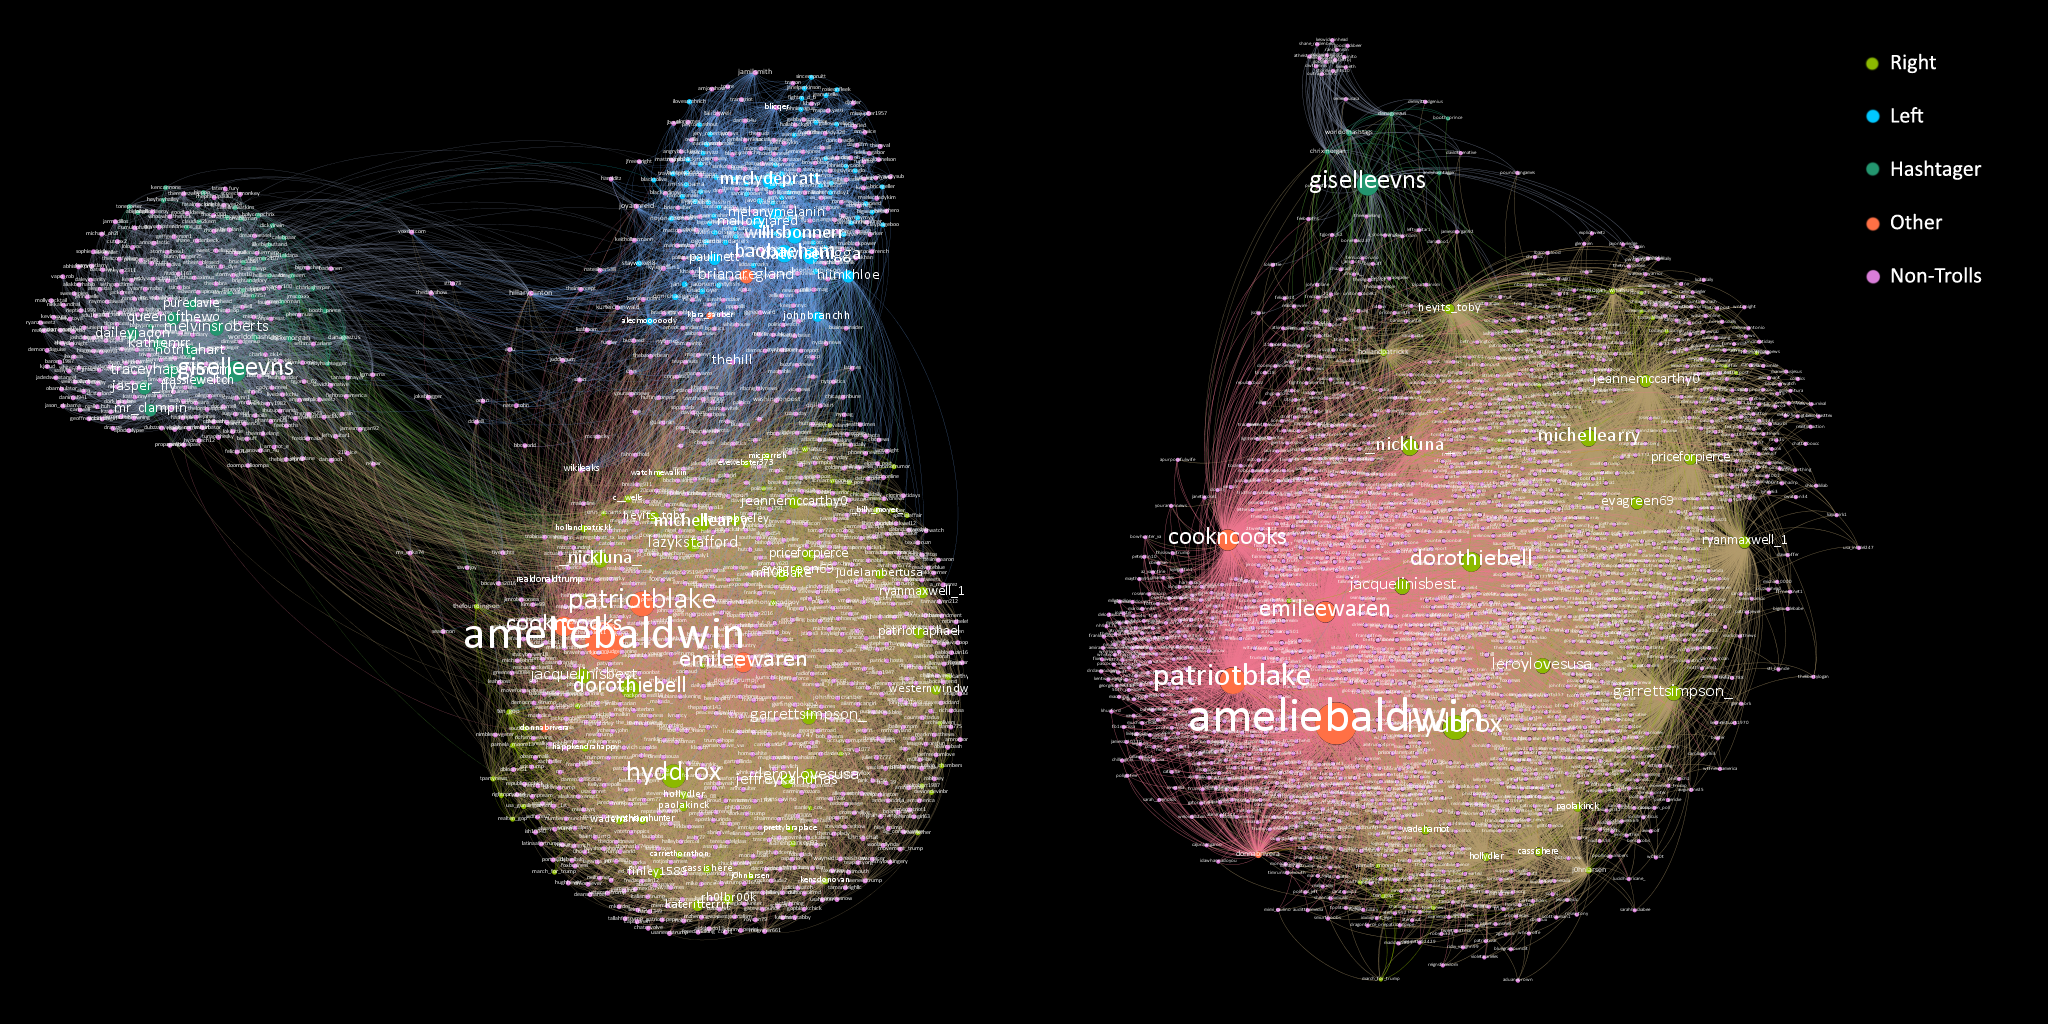
\includegraphics[width=0.95\linewidth]{final_k_graphs.png}
\caption[k-core and k-in-core]{k-10-core and k-in-4-core. Node and label size represent outdegree centrality, colors reflect community.}
\label{fig:kcore}
\end{figure}

Since the k-in-core consists mostly of right-wing accounts, a further analysis of the k-10-core seems to be more fruitful. The accounts in the k-10-core are those with the best positions in the network regarding the ability to spread information. We therefore proceed to examine the most active accounts, since they can be considered as the most influential. Figure~\ref{fig:k10in} provides an overview of the 30 accounts with the highest outdegree within the k-10-core, and thus the profiles who retweeted the relevant accounts most often. The profile \textit{ameliebaldwin} has by far the largest outdegree, putting this account at the central position of the core. Interestingly, of the top 6 profiles, 4 were categorized as \textit{Other} by the community detection algorithm. Looking on Figure~\ref{fig:kcore}, they all are very close to the right-wing community (the same is true for the k-in-core). Linvill and Warren categorized most of them as right-wing as well, which indicates some inaccuracy of the community detection algorithm, i.e. it is to sharp, thus detecting too many communities. Seeing them as right-wing shows a very clear dominance of right-wing profiles concerning information super-spreaders, which is consistent with the previous findings.

\begin{figure}[!ht]
\centering
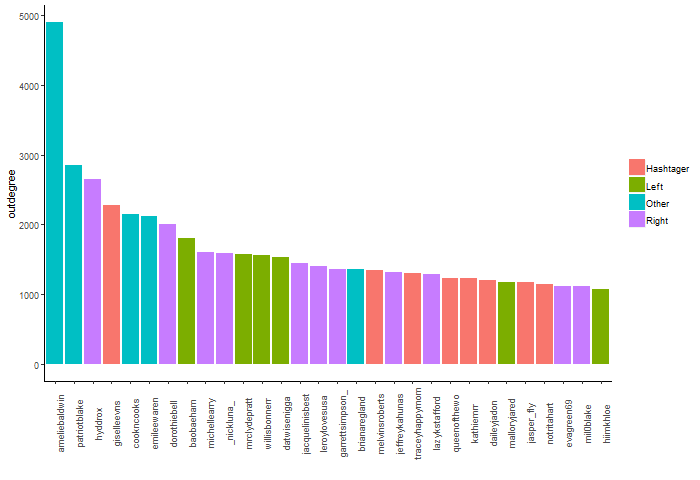
\includegraphics[width=0.95\linewidth]{k10_figure}
\caption[Outdegree in the k-core]{Top 30 user regarding outdegree in the k-10-core.}
\label{fig:k10in}
\end{figure}


\subsection{Discussion}

Our analysis shows that the IRA did not only conduct astroturfing for one single community, but for at least three distinct social groups on Twitter. Targeting all of them ensured broader influence, especially considering the selection of left- and right-wing communities, suggesting a strategy to enhance an already present divide in society. We can therefore verify Linvill and Warren's qualitative findings out of the structure of the network itself. The community detection results in a distribution of the right-wing cluster into two smaller communities. We can only speculate this being due to the right-wing's division into subgroups e.g. conservatives and alt-right. Another possibility is the relatively small size or the ego-centered nature of our network leading to the algorithm detecting more communities. An interesting finding is the IRA's targeting of the \textit{Hashtag Gamer} community, since they are not known for their wide political influence. Again, we can only speculate since they are a relatively well connected group, meaning information ca be spread well through their channels. Adding Linvill and Warren's findings, the IRA might have tried to politicize this group to widen the scope of their astroturfing to a big, well-connected, but not very politically active twitter community.
\marginpar{OF}

Comparing the three communities, the IRA put a definite focus on the right-wing community. Right troll accounts are retweeting more regarding the mere quantity, as well as the range of different accounts retweeting. Accounts in the left community are less connected and tend to repeatedly retweet the same accounts very often. It is unclear, whether this is intentional IRA behavior or it is based in the way those communities function differently. Although we can assume that it to be intentional, since statements of Lyudmila Savchuk (\cite{savchuk_inside_2018}), an investigative journalist who worked for a couple of months undercover for the IRA, indicate that every tweet was seen through before posting. Due to the nature of the \textit{Hashtag Gamers} community they appear to be the most connected. 

The IRA's focus on the right-wing community is reinforced through those accounts mainly retweeting themselves, while user from the other communities do retweet right-wing accounts. Again, we can only assume, this is intentional and not based in the community structure. Weather intentional or not, the IRA was definitely more active and able to spread information broader within and from the right-wing community. The analysis of the k-10-core and the k-in-4-core locates the super-spreaders of information mostly in the right-wing community as well, which is no surprise considering the fact that this community is retweeted by everyone else. The most active troll account in the most connected core of the network is by far \textit{ameliebaldwin}. It is unclear why exactly this account has such a key position, while the other super-spreaders are relatively close to each other, suggesting a division of labor between those accounts. Although the focus is on the right-wing community, left-wing and \textit{Hastag Gamer} accounts are not unimportant, some of them occupying considerable central positions, but to a lesser degree than right-wing trolls.

The most prestigious accounts, meaning the accounts retweeted by the most trolls, range from accounts of important politicians like President Trump or Hillary Clinton through big news channels like \textit{The Hill} or \textit{Fox News} to political journalists like Joy Reid or Jamil Smith. This makes sense, since those profiles have a lot of followers and people are referring to them very often. In regards to the total amount of retweets, this would suggest those profiles to also be the most prestigious when considering the total amount of retweets. However, with the exception of President Trump, other profiles take their spot. In our dataset it appears that \textit{blicqer}, a black activist user, operates the account with the most retweets. The second being \textit{conservatexian}, a right-wing user. Both stand as prime examples for users of the left and right communities: both are big profiles, but not official government or news accounts. It suggests that the IRA rather shares information from unofficial accounts which do not employ standards regarding information checking before they tweet.

This study had to deal with some severe limitations regarding the available data, the network being ego-centered being the main obstacle, since it allows for less interpretation. While we have a lot of information on the trolls' own retweet behavior, we do not know which troll has been retweeted how much by non-troll users, leaving us with fewer possibilities than with a complete non-ego-centered network (e.g. the number of regular tweets of accounts as a node attribute or ratios of how many retweets per tweet a user is receiving can enhance the analysis). We cannot presume that the indegree of a troll account is a good measure for the actual number of retweets an account gets, since non-troll retweet behavior could be completely different from troll activity on Twitter. It is important to highlight, that a complete network of the same nodes would presumably change the structure of the graph, including centralities and community allocation. This implies that our graph does not tell us the actual positions of the nodes in the complete Twitter network. With a bigger and thus more representative dataset, the smaller communities of trolls we categorized as other would be represented accurately and could be analyzed. Our graph mainly is a depiction of how the group of trolls constituting our dataset interacted with each other and whose tweets they chose to spread. Outdegree centralities and the k-core measure are therefore eligible to compare trolls or groups of trolls with each other. According to this, our findings appear to be valid within the scope of an ego-centered network. Although we rely on the assumption that there is no substantial group of trolls missing, which might skew the results regarding a community comparison.
\marginpar{JK}


\section{Conclusion}

Distinguishing true from false information becomes increasingly difficult in today's social media landscape. In this paper, we tried to shed some light on the structure and strategy of the organized disinformation campaign of the IRA. Situating their behavior in astroturfing as a strategy for agenda building, we showed how they target specific communities on Twitter, in order to create the impression of a certain public opinion as diametrical opposed. We have explored the division of labor of different troll accounts, as well as their positions within a retweet network. Instead of creating the impression of one social movement, the IRA is operating within different, even opposed communities, while focusing on the right-wing community. With one exception, they have a couple of accounts in central positions spreading mainly (dis-)information regarding political topics. Hence, we can confirm, that the problem of disinformation campaigns cannot be solved, only marginally improved, by banning some highly influential accounts, even if examples like \textit{ten\_gop} might suggest otherwise. Interestingly, our results show the IRA trying to influence the not distinctly political, but well connected community of \textit{Hashtag Gamers}. If organizations like the IRA specifically target non-political communities, the problem of agenda-building through disinformation campaigns is even bigger than assumed right now.
\marginpar{OF}

Although the dataset used in this paper posed some severe limitations -- especially the dataset consisting of only tweets from the troll accounts, which resulted in the network being ego-centered, as well as it not being complete -- we were able to highlight central aspects of the strategies of the IRA. Thus, we demonstrated the merits of SNA in exploring strategies of organizations conducting disinformation campaigns, while having no possibility to learn of their intentions through other social science methods like interviews. The methodological approach of SNA, which takes structures as a starting point makes it the prime tool for cases like this, even if the data is incomplete. That being said, to fully understand how organizations like the IRA work, much more research is needed. Especially with a more complete dataset, that does not result in just a retweet network, a SNA can deliver more valid results. This study pointed to some further questions regarding the functioning of communities on Twitter. Here, more sociological knowledge can help identifying weather the IRA's different retweet structure in different communities is strategic or rooted in those communities themselves, e.g. through an analysis of different trending hashtag discussions, which could shed light on how specific community behavior might change between policy areas. The question why some troll accounts have much more output also should be discussed. Lastly, it can be learned a lot from comparing cases. Astroturfing is no new phenomenon, accordingly compare the IRA with similar agencies can give a better understanding of how these operate. Taking one step back, SNA does not necessarily have to be conducted via a network of retweets, but could also be done with mentions.\footnote{Mentions mean the tagging of another user's name without spreading information of their tweet.} Contrary to retweets, mentions appear to be more easily used to contradict another user, which would make the ties a lot harder to define and interpret, but an interesting choice for comparing a network drawn from the same data.

All in all, influencing and agenda-building poses a big problem, especially for democratic states, since social media here reaches very far into society. Right now organizations like the IRA have the advantage, because they were able to operate out of the dark. But through in-depth research happening right now, of which this paper is only a marginal part, we can analyze their structure and strategies and thus hopefully find the necessary tools to prevent disinformation campaigns from reaching considerable impact.


\newpage

\printbibliography


\end{document}
